\RequirePackage[ngerman=ngerman-x-latest]{hyphsubst}

\documentclass[
    bibliography=totoc, cd=lightcolor, cdmath=false, ngerman]{tudscrreprt}

\usepackage[Algorithmus]{algorithm}
\usepackage{algpseudocode}
\usepackage{amsmath}
\usepackage{amssymb}
\usepackage[german]{babel}
\usepackage{caption}
\usepackage{chngcntr}
\usepackage[T1]{fontenc}
\usepackage{hyperref}
\usepackage[utf8]{inputenc}
\usepackage{mathtools}
\usepackage{minted}
\usepackage{pxfonts}
\usepackage{subcaption}
\usepackage[dvipsnames]{xcolor}

% import after xcolor to avoid clash
\usepackage{lstlinebgrd}
\usepackage{svg}
\usepackage{tikz}
\usetikzlibrary{arrows.meta,backgrounds,chains,decorations.pathreplacing}

% misc settings
\counterwithin{listing}{chapter}

\DeclarePairedDelimiter\ceil{\lceil}{\rceil}

\setminted{%
  frame=single,
  fontsize=\scriptsize,
  labelposition=none,
  linenos=true
}
\tikzset{%
  TikzStyle/.style={draw,minimum width=30pt,minimum height=20pt,font=\small}
}

\begin{document}

\title{Komplexpraktikum Paralleles Rechnen}

\author{
  Timo Nicolai
  \course{Informationssystemtechnik}
  \matriculationnumber{4048209}
}

\supervisor{Dipl.-Ing. Oliver Knodel}

\headingsvskip=-100pt

\maketitle
\tableofcontents
\pagebreak

\chapter{Einleitung}
Dieser Beleg beschreibt die Implementierung von Lloyds k-means
Vektorquantisierungs-Algorithmus sowohl in serieller als auch parallelisierter
Form.

Die Parallelisierung wurde zum einen durch parallele Nutzung mehrerer
Prozessor-Kerne mittels \texttt{OpenMP} Quellcode-Annotationen und zum anderen
durch Auslagerung parallelisierbarer Performance-kritischer Abschnitte auf eine
\texttt{NVIDIA}-GPU mittels \texttt{CUDA} erreicht. Beide Methoden werden im
Folgenden mit Hinblick auf Besonderheiten in der Implementierung und
Performance-Gewinnen in Abhängigkeit der Problemgröße und genutzten
Hardware-Ressourcen mit der seriellen Implementierung gegenübergestellt.

\chapter{Der k-means Algorithmus}

\section{Beschreibung des Algorithmus}

Unter der Bezeichnung k-means sind mehrere Algorithmen bekannt, die alle zum
Ziel haben, auf effizientem Wege eine annähernde Lösung für das folgende Problem
zu finden:
\bigbreak
Eine Menge von Vektoren ist derart in $k$ Partitionen zu zerlegen, dass die
Summe der quadratischen euklidische Distanzen aller Vektoren in jeder Partition
zum jeweiligen Partitions-Schwerpunkt minimiert wird. D.h. sei $M$ eine Menge
von Vektoren $x \in \mathbb{R}^n$, dann sind Partitionen $P = \{P_i \mid i =
1,2,\dots,k\}$ von $M$ mit Schwerpunkten $S = \{\mu_i \mid i = 1, 2, \dots,
k\}$ gesucht, sodass der folgende Ausdruck minimal wird:
$$
\sum_{k} \sum_{x \in P_k} ||x - \mu_k||^2
$$
Der hier betrachtete Algorithmus ist wohl der bekannteste und einfachste unter
diesen Algorithmen und wurde erstmals von Lloyd vorgeschlagen \cite{bib:lloyd}.
Er basiert auf der wiederholten Zuweisung von Vektoren zu den Partitionen mit
den ihnen am nähsten gelegenen Schwerpunkten und folgender Neuberechnung dieser
Schwerpunkte und ist hier als Algorithmus~\ref{alg:lloyd} dargestellt.

\begin{algorithm}
    \caption{Llyods k-means Algorithmus}
    \begin{algorithmic}[1]
        \Procedure{k-means}{$x$}
            \State // Initialisiere Schwerpunkte mit zufälligen Vektoren
            \For{$i = 1 \dots k$}
                \State $P_i := \emptyset$
                \State $\mu_i := \text{ein zufälliges } x_j \in M$
            \EndFor
            \State // Berechne (annähernd) ideale Partitionen iterativ
            \While{Änderungen an $P$} \label{alg:loop_begin}
                \State // Weise Vektoren den Partitionen mit nächstem Schwerpunkt zu
                \For{$x_i \in M$} \label{alg:cluster_begin}
                    \State $j := \mathrm{argmin}_j\ ||x_i - \mu_j||$
                    \State $P_j := P_j \cup \{x_i\}$
                \EndFor \label{alg:cluster_end}
                \State // Aktualisiere Partitions-Schwerpunkte
                \For{$i = 1 \dots k$}
                    \State $\mu_i := |P_i|^{-1} \sum_{x_j \in P_i} x_j$
                \EndFor
            \EndWhile \label{alg:loop_end}
        \EndProcedure
    \end{algorithmic}
    \label{alg:lloyd}
\end{algorithm}

Es ist zusätzlich zu beachten, dass es mehrere denkbare Bedingungen für den den
Abbruch der Hauptschleife in den Zeilen \ref{alg:loop_begin} bis
\ref{alg:loop_end} geben kann. Die in Algorithmus~\ref{alg:lloyd} gezeigte
triviale Abbruchbedingung greift dann, wenn in einer Iteration kein Vektor die
Partition wechselt. In diesem Fall wurde eine stationäre Lösung gefunden und
die Berechnung kann abgebrochen werden. Auch möglich ist es, von vorneherein
ein Limit für die Anzahl der Iterationen festzulegen bei dessen Überschreitung
abgebrochen wird auch wenn keine stationäre Lösung gefunden wurde. Eine weitere
Möglichkeit ist es, dann abzubrechen wenn sich in einer Iteration keiner der
Partitions-Schwerpunkte um mehr als einen Schwellwert $\epsilon$ von seinem
vorherigen Wert entfernt. In den folgenden Implementierungen wird stets mit
einem Iterations-Limit von 100 gearbeitet (das praktischen Untersuchungen nach
jedoch selten erreicht wird).

Außerdem ist in Algorithmus~\ref{alg:lloyd} die Behandlung leer verbliebener
Partitionen nach der Schleife in den Zeilen \ref{alg:cluster_begin} bis
\ref{alg:cluster_end} nicht dargestellt. Dieser Fall sollte in einer
``vernünftigen'' Implementierung für die meisten Inputs eher die Ausnahme als
die Regel darstellen, muss aber trotzdem berücksichtigt werden um die
Korrektheit des Algorithmus zu garantieren. Der in den folgenden
Implementierungen (mit Ausnahme der \texttt{CUDA C} Implementierung) gewählte
Ansatz ist es, iterativ alle leeren Partitionen mit dem Vektor aus der jeweils
momentan größten Partition, der von deren Schwerpunkt am weitesten entfernt
ist, zu füllen.

Der Algorithmus wie er hier dargestellt ist, kann auf Mengen von Vektoren
beliebiger Dimensionen angewandt werden. Im Folgenden wird allerdings nur noch
die Anwendung des k-means Algorithmus zur Segementierung von Farbbildern
betrachtet (und somit der Fall $x \in F \subset \mathbb{R}^3$ unter der
Annahme, dass $M$ die Menge aller Pixel eines Bildes in
\texttt{RGB}-Vektordarstellung und $F$ der \texttt{RGB}-Farbraum ist, d.h. $x =
(r, g, b)^T$ mit $r, g, b \in [0, 255])$.

\section{Sequentielle Implementierung}

Listing~\ref{lst:kmeansc} zeigt eine sequentielle Implementierung des k-means
Algorithmus in C. Die Funktion \texttt{kmeans} in Zeile 42 zerlegt die
\texttt{n\_pixels} in \texttt{pixels} gespeicherten Pixel in
\texttt{n\_centroids} Partitionen mit den Schwerpunkten \texttt{centroids}. Die
Funktion weist zu diesem Zweck jedem Pixel \texttt{pixels[i]} in
\texttt{labels[i]} den Index der Partition zu der dieser Pixel gehört zu.
\texttt{struct pixel} repräsentiert dabei einen Punkt im \texttt{RGB}-Farbraum
und ist wie in Listing~\ref{lst:structpixel} gezeigt definiert.

\captionof{listing}{%
Sequentielle k-means Implementierung in C (Ausschnitt \texttt{kmeans.c})
\label{lst:kmeansc}}
\inputminted[lastline=203, label=kmeansc]{C}{c/src/kmeans.c}

\captionof{listing}{struct pixel (Ausschnitt \texttt{kmeans.h})
\label{lst:structpixel}}
\inputminted[firstline=4, lastline=7]{C}{c/include/kmeans.h}

Will man die Funktion nutzen um ein Farbbild zu segmentieren, muss man also
zunächst die Pixel des Bildes in ein eindimensionales Array vom Typ
\texttt{struct pixel[]} transformieren und der Funktion \texttt{kmeans}
übergeben. Danach kann dann der jeweils i-te Pixel durch den in
\texttt{centroids[labels[i]]} gespeicherten Schwerpunkt der Partitionen der er
zugeteilt wurde ersetzt und anschließend das zweidimensionale Bild
rekonstruiert werden.

In den Zeilen 61-68 findet die zufällige Initialisierung der
Partitions-Schwerpunkte statt. Die Hauptschleife in den Zeilen 71-192 iteriert
solange, bis keine Neuverteilung von Pixeln auf Partitionen mehr stattfindet
oder \texttt{KMEANS\_MAX\_ITER} Iterationen erreicht worden sind. Dabei werden
in den Zeilen 78-100 alle Pixel den Partitionen mit dem ihnen am nächsten
liegenden Schwerpunkt zugewiesen. Gleichzeitig werden die Summen aller Pixel in
jeder Partition im Array \texttt{sums} und die Größen der Partitionen im Array
\texttt{counts} festgehalten. In den Zeilen 109-161 wird die (verhältnismäßig
aufwändige aber in den meisten Anwendungsfällen selten auftretende)
Umverteilung von Pixeln auf eventuell leer gebliebene Partitionen vorgenommen.
In Zeilen 170-184 werden die neuen Schwerpunkte über die in \texttt{sums} und
\texttt{counts} gepeicherten Werte berechnet.

\subsection{Profiling}
Vor der Parallelisierung der Implementierung ist es sinnvoll zunächst zu
bestimmen welche Codeabschnitte am meisten zur Gesamtlaufzeit des Algorithmus
beitragen. Diese sollten dann entsprechend bei der Parallelisierung priorisiert
werden (sofern sie sinnvoll parallelisierbar sind). Wird das gezeigte Programm
mit gesetztem \texttt{PROFILE} Symbol kompiliert, so wird für die drei
wichtigsten Programmabschnitte (zuweisen von Pixeln zu Partitionen, Reparatur
leerer Partitionen und Neuberechnung der Partitions-Schwerpunkte) jeweils die
CPU-Laufzeit (hier aufgrund fehlender Parallelisierung quasi identisch zur
``wall-clock-time'') aufgezeichnet und auf der Konsole ausgegeben (z.B. mittels
\texttt{make profile}).  Auf ein Beispielbild
(\texttt{images/profile\_image.jpg, 512$\times$512 Pixel}) angewandt ergeben
sich so beispielsweise folgende Werte:

\inputminted[linenos=false]{text}{report/resources/profiling.txt}

Es ist hier nicht überraschend, dass die Neuzuweisung von Pixeln an die
Partitionen mit den ihnen am nächsten liegenden Schwerpunkten um einige
Größenordnungen mehr Zeit beansprucht als die beiden anderen Abschnitte.  Die
Reparatur findet für typische Inputs sehr selten bzw. gar nicht statt und die
Neuberechnung der Schwerpunkte ist mit wenig Rechenaufwand verbunden. Diese
beiden Abschnitte sind für die erfolgreiche Parallelisierung demnach quasi
irrelevant.

\chapter{Parallelisierung}

\section{OpenMP}

\subsection{Implementierung}

Listing~\ref{lst:kmeansomp} zeigt die mittels \texttt{OpenMP} parallelisierte
Variante der in Listing~\ref{lst:kmeansc} gezeigten C-Implementierung.
Modifizierte Zeilen sind farbig hervorgehoben. Es mussten nur einige wenige
Änderungen vorgenommen werden um eine performante Parallelisierung zu
erreichen. Hier zeigt sich eine große Stärke von OpenMP: existierender Code
kann teilweise (fast) ohne Änderungen am Code selbst nur durch die Nutzung von
\texttt{\#pragma} Direktiven parallelisiert werden.  Natürlich muss für
maximale Ausnutzung der dem Algorithmus inhärenten Parallelisierbarkeit eine
günstige Code-Struktur vorliegen. Dies ist hier aber prinzipiell schon gegeben,
da die Performance-kritische Schleife in Zeilen 78-100 in
Listing~\ref{lst:kmeansc} bereits in geigneter Form vorliegt.  Hier können die
Berechnungen für jedes Pixel unabhängig voneinander erfolgen, es muss lediglich
der Zugriff auf die Variable \texttt{done}, \texttt{sums} und \texttt{counts}
synchronisiert werden. Für erstere genügt eine \texttt{\#pragma atomic write}
Direktive, für die beiden Arrays kann die \texttt{reduction} Klausel
\footnote{Seit OpenMP Version 4.5 (z.B. von GCC ab Version 6.1 unterstützt) auf
Arrays anwendbar.} genutzt werden. Hierfür muss dann allerdings \texttt{sums}
als Array von Fließkommazahlen realisiert werden.  (jeweils drei aufeinander
folgende ersetzen ein \texttt{struct pixel}) da Reduktionen nicht auf
nutzerdefinierte Typen angewandt werden können.

Andere Abschnitte des Algorithmus können potentiell ebenfall parallelisiert
werden, allerdings mit vergleichbar kleinem Performance-Gewinn. Bei der
Reparatur leerer Partitionen wurde ebenfalls über die einzelnen Pixel
parallelisiert, dieser Codeabschnitt wird jedoch nur selten (wenn überhaupt)
aufgerufen. Eine Parallelisierung bei Neuberechnung der Schwerpunkte
hat für realistische Input-Größen keinen starken Einfluss auf die
Ausführungszeit des Programms ist hier aber ebenfalls einfach möglich.

\captionof{listing}{Parallelisierte k-means Implementierung mit \texttt{OpenMP}
(Ausschnitt \texttt{kmeans.c})\label{lst:kmeansomp}}
\inputminted[firstline=207, label=kmeansomp, highlightlines={
215, 222-223, 233-234, 246, 251-254, 286, 293-294, 299, 308-311, 313-316, 324,
327, 330-332, 334}]{C}{c/src/kmeans.c}

\subsection{Performance}

Abbildung~\ref{img:cboxplot} und Abbildung~\ref{img:ompboxplot} visualisieren
die Ausführungszeiten des seriellen sowie des mit \texttt{OpenMP}
parallelisierten k-means Algorithmus (hier bei Nutzung aller Prozessor-Kerne).

Für alle auf der horizontalen Achse abgetragenen Bild-Dimensionen wurden beide
Implementierungen auf je 100 verschiedene, zufällig generierte Farbbilder
angewandt. Die Programme wurden auf einer Maschine mit einem \texttt{Intel Core
i5D-4690} Prozessor mit vier Prozessor-Kernen getestet. Die Boxplots lassen
erkennen, in welchem Bereich sich die Ausführungszeiten jeweils befinden und
wie groß ihre Streuung ist. Die gestrichtelte Linie verläuft durch die Mediane
der Ausführungszeiten und zeigt wie zu erwarten in beiden Fällen eine lineare
Abhängigkeit der Ausführungszeit von der Anzahl der Pixel auf.

Abbildung~\ref{img:compspeedup} zeigt für dieselben Bild-Dimensionen jeweils
den Durchschnitt des durch die Nutzung von \texttt{OpenMP} erreichten Speedup.
Es lässt sich erkennen, dass für angemessene Problemgrößen ein Speedup, der
ungefähr im Bereich der Anzahl der zur Verfügung stehenden Prozessorkerne
\footnote{Jeweils mittels \texttt{omp\_set\_num\_threads()} konfiguriert.},
wobei der Geschwindigkeitsgewinn mit steigender Prozessoranzahl jedoch immer
kleiner ausfällt. Gleichzeitig ist bei Nutzung von mehreren Kernen die
Schwankung der Ausführungszeiten größer.

\begin{figure}[htbp]
  \centering
    \includesvg[width=0.8\textwidth]{report/resources/C_boxplot}
  \caption{Serielle C Implementierung - Ausführungszeiten \\
           (je 100 Datenpunkte pro Bild-Dimension)}
  \label{img:cboxplot}
\end{figure}

\begin{figure}[htbp]
  \centering
    \includesvg[width=0.8\textwidth]{report/resources/OpenMP_quad_boxplot}
  \caption{Parallelisierte OpenMP Implementierung - Ausführungszeiten \\
           (vier Prozessorkerne, je 100 Datenpunkte pro Bild-Dimension)}
  \label{img:ompboxplot}
\end{figure}

\begin{figure}[htbp]
  \centering
    \includesvg[width=0.8\textwidth]{report/resources/C_OMP_speedup}
  \caption{Speedup C vs. C + OpenMP}
  \label{img:compspeedup}
\end{figure}

\section{CUDA}

\subsection{Implementierung}

Listing~\ref{lst:kmeanscuda} zeigt die mittels \texttt{CUDA} parallelisierte
Version des Programms. Im Gegensatz zur \texttt{OpenMP} Variante unterscheidet
diese sich deutlich vom reinen C-Code. Die Performance kritische Zuweisung von
Pixeln zu Partitionen sowie die Neuberechnung der Schwerpunkte sind mittels auf
der Grafikkarte (nachfolgend \texttt{Device}) ausgeführten \texttt{Kerneln}
realisiert (letzterer dient hauptsächlich dazu unnötiges Übertragen von
Zwischenergebnissen von Device zu Host zu vermeiden). Beide Kernel sind so
geschrieben, dass sie prinzipiell mit einer beliebigen Anzahl von Blöcken und
Threads ausgeführt werden können, die Implementierung nutzt jedoch eine
konstante Zahl von Threads und wählt die Zahl der Blöcke sinnvoll in
Abhängigkeit der Größe des Input Pixel-Arrays.

\captionof{listing}{%
Parallelisierte k-means Implementierung mit \texttt{CUDA} (kmean.cu)
\label{lst:kmeanscuda}}
\inputminted[label=kmeanscuda]{CUDA}{c/src/kmeans.cu}

Die Parallelisierung ist hier von der Struktur her sehr ähnlich zu der bereits
mit \texttt{OpenMP} realisierten. Problematisch ist hier nur, dass
\texttt{CUDA} kein zu \texttt{OpenMP} äquivalente Syntax zur automatischen
Reduktion von Arrays bietet. Diese musste dementsprechend in
den \texttt{reassign} und \texttt{average} Kerneln explizit implementiert
werden.

Der \texttt{reassign} Kernel lädt zunächst in Zeile 49 die Schwerpunkte in ein
\texttt{shared memory} Segment, um den wiederholten lesenden Zugriff aller
Threads in diesem Block auf die Schwerpunkte zu beschleunigen. In den Zeilen
64-90 wird anschließend äquivalent zur \texttt{OpenMP}-Implementierung pro
Thread der zu einem Pixel nächste Schwerpunkt ermittelt. In Zeile 92 beginnt
dann die Reduktion welche die \texttt{sums} und \texttt{counts} Arrays
aktualisiert und die Nutzung kritischer Abschnitte umgeht. Dabei wird der
gleiche Reduktionsschritt sequentiell auf die einzelnen Partition angewandt.
Anschließend haben die Bereiche globalen Device-Speichers auf die \texttt{sums}
bzw. \texttt{counts} (im Kernel, nicht zu verwechseln mit den gleichnamigen
Host-Zeigern) zeigen folgenden Inhalt:

\vspace{10pt}

\begin{tikzpicture}
  \begin{scope} [start chain, node distance=-.5pt]
    \foreach \name [count=\xi] in {
      \ \ sums[0]\ \ ,\cdots,sums[k-1],
      \cdots,\cdots,\cdots,
      \ \ sums[0]\ \ ,\cdots,sums[k-1]
    }{ \node[TikzStyle,on chain,font=\small] (n\xi) {$\name$};}
  \end{scope}
  \node[above= 0.1cm of n1, xshift=-0.5cm]{$sums$};
  \draw [decorate,decoration={brace,amplitude=10pt,mirror}]
  (n1.south west) -- (n3.south east) node[black,midway,below=8pt]{$block\ 0$};
  \draw [decorate,decoration={brace,amplitude=10pt,mirror}]
  (n7.south west) -- (n9.south east) node[black,midway,below=8pt]
  {$block\ \ceil*{\frac{|M|}{|Threads|}}$};
\end{tikzpicture}

\begin{tikzpicture}
  \begin{scope} [start chain, node distance=-.5pt]
    \foreach \name [count=\xi] in {
      \ \ counts[0]\ \ ,\cdots,counts[k-1],
      \cdots,\cdots,\cdots,
      \ \ counts[0]\ \ ,\cdots,counts[k-1]
    }{ \node[TikzStyle,on chain] (n\xi) {$\name$};}
  \end{scope}
  \node[above= 0.1cm of n1, xshift=-0.5cm]{$counts$};
  \draw [decorate,decoration={brace,amplitude=10pt,mirror}]
  (n1.south west) -- (n3.south east) node[black,midway,below=8pt]{$block\ 0$};
  \draw [decorate,decoration={brace,amplitude=10pt,mirror}]
  (n7.south west) -- (n9.south east) node[black,midway,below=8pt]
  {$block\ \ceil*{\frac{|M|}{|Threads|}}$};
\end{tikzpicture}

\vspace{10pt}

D.h. es existiert dann in diesen Speicherbereichen pro Block für den der Kernel
ausgeführt worden aneinandergereiht Arrays deren Dimensionen bereits denen der
Host-Speicherbereichen auf die die Host-Zeiger \texttt{sums} und
\texttt{counts} zeigen entsprechen und die jeweils den Beitrag aller in dem
jeweiligen Block betrachteten Pixeln darstellen.

Die Reduktion erfolgt dabei für beide Arrays in
$log_2\left(\left|Threads\right|\right)$ Schritten. Dabei wird zunächst in
Zeilen 94-101 im \texttt{shared memory} Segment für jeden Thread genau dann
wenn der für den zum Thread gehörige Pixel bestimmte nächstgelegene Schwerpunkt
in der aktuell betrachteten Partition liegt dessen Wert und eine eins (für die
Bestimmung der Partitionsgröße) im \texttt{shared memory} Segment abgelegt.
Anschließend werden diese Werte nach folgendem Schema schrittweise addiert um
die entsprechenden Werte für den gesamten Block zu erhalten (hier
beispielsweise für acht Threads pro Block):

\vspace{20pt}

\begin{tikzpicture}
\foreach \x in {0,...,7} {
    \node (n\x0) [TikzStyle,minimum width=50pt] at (2*\x,0) {Thread \x};
}

\node (n01) [TikzStyle,minimum width=50pt,font=\scriptsize] at (0,-4) {Thread 0,4};
\node (n11) [TikzStyle,minimum width=50pt,font=\scriptsize] at (2,-4) {Thread 1,5};
\node (n21) [TikzStyle,minimum width=50pt,font=\scriptsize] at (4,-4) {Thread 2,6};
\node (n31) [TikzStyle,minimum width=50pt,font=\scriptsize] at (6,-4) {Thread 3,7};
\node (n02) [TikzStyle,minimum width=50pt,font=\tiny] at (0,-8) {Thread 0,2,4,6};
\node (n12) [TikzStyle,minimum width=50pt,font=\tiny] at (2,-8) {Thread 1,3,5,7};
\node (n03) [TikzStyle,minimum width=50pt] at (0,-12) {Block};

\node (p1) [TikzStyle,circle] at (0,-2.5) {+};
\node (p2) [TikzStyle,circle] at (2,-2.5) {+};
\node (p3) [TikzStyle,circle] at (4,-2.5) {+};
\node (p4) [TikzStyle,circle] at (6,-2.5) {+};
\node (p5) [TikzStyle,circle] at (0,-6.5) {+};
\node (p6) [TikzStyle,circle] at (2,-6.5) {+};
\node (p7) [TikzStyle,circle] at (0,-10.5) {+};

\begin{scope}[on background layer]
    \draw [-{Stealth[scale=1.5]}] (n00.south) -- (p1.north);
    \draw [-{Stealth[scale=1.5]}] (n10.south) -- (p2.north);
    \draw [-{Stealth[scale=1.5]}] (n20.south) -- (p3.north);
    \draw [-{Stealth[scale=1.5]}] (n30.south) -- (p4.north);
    \draw [-{Stealth[scale=1.5]}] (n40.south) -- (p1.north);
    \draw [-{Stealth[scale=1.5]}] (n50.south) -- (p2.north);
    \draw [-{Stealth[scale=1.5]}] (n60.south) -- (p3.north);
    \draw [-{Stealth[scale=1.5]}] (n70.south) -- (p4.north);
    \draw [-{Stealth[scale=1.5]}] (p1) -- (n01);
    \draw [-{Stealth[scale=1.5]}] (p2) -- (n11);
    \draw [-{Stealth[scale=1.5]}] (p3) -- (n21);
    \draw [-{Stealth[scale=1.5]}] (p4) -- (n31);
    \draw [-{Stealth[scale=1.5]}] (n01.south) -- (p5.north);
    \draw [-{Stealth[scale=1.5]}] (n11.south) -- (p6.north);
    \draw [-{Stealth[scale=1.5]}] (n21.south) -- (p5.north);
    \draw [-{Stealth[scale=1.5]}] (n31.south) -- (p6.north);
    \draw [-{Stealth[scale=1.5]}] (p5) -- (n02);
    \draw [-{Stealth[scale=1.5]}] (p6) -- (n12);
    \draw [-{Stealth[scale=1.5]}] (n02.south) -- (p7.north);
    \draw [-{Stealth[scale=1.5]}] (n12.south) -- (p7.north);
    \draw [-{Stealth[scale=1.5]}] (p7) -- (n03);
\end{scope}
\end{tikzpicture}

\vspace{20pt}

Im \texttt{average} Kernel findet weiterer ähnlicher Reduktionsschritt statt
der diese Arrays aufsummiert und so die gewünschten Partitions-Summen und
Größen ermittelt mit deren Hilfe dann die neuen Partitions-Schwerpunkte
berechnet werden.

Dieser Ansatz umgeht zwar den Einsatz atomarer Operation und kritischer
Abschnitte die seriell abgearbeitet werden müssen und damit zu starken
Performance-Einbußen führen, resultiert aber trotzdem durch die vielen
benötigten Thread-Synchronisations-Punkte nicht in einer optimalen GPU
Auslastung. Mit \texttt{NVIDIA Nsight} lässt sich ermitteln, dass rund die
Hälfte aller auftretenden Instruction Stalls durch Thread-Synchronisation
bedingt sind.

Außerdem limitiert der relativ hohe Shared Memory Bedarf zu Beginn
jedes Reduktionsschrittes die Anzahl parallel ausführbarer Warps pro Streaming
Multiprocessor, wie in Abbildung~\ref{fig:shm} (ebenfalls mit Nsight ermittelt)
zu erkennen ist.

\begin{figure}[htbp]
  \begin{center}
    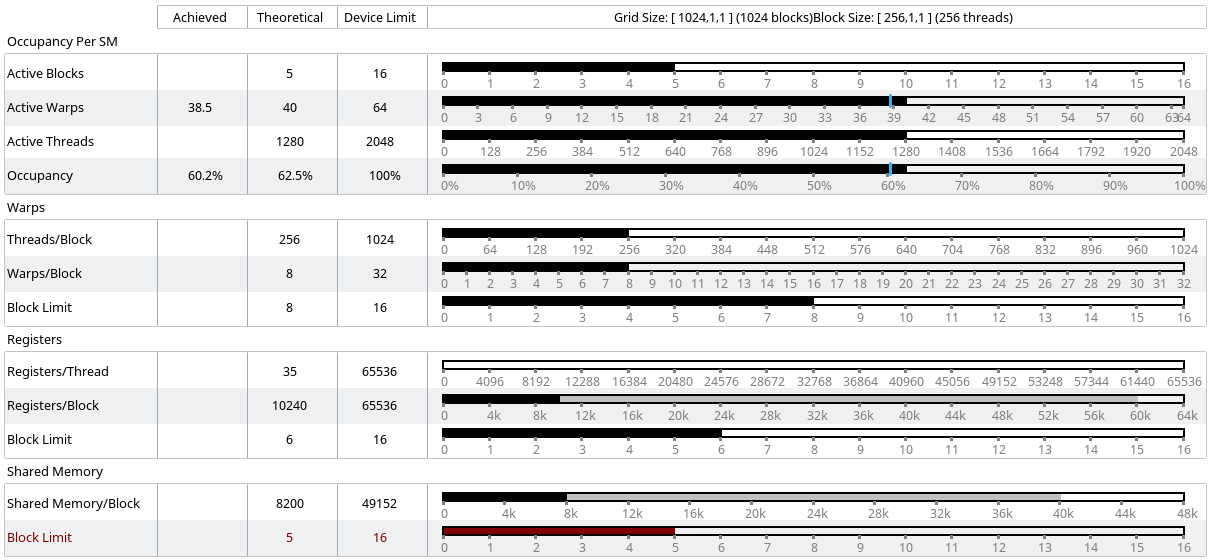
\includegraphics[width=\textwidth,keepaspectratio]{%
    report/resources/shm_usage.png}
  \end{center}
  \caption{Shared Memory Ausnutzung}
  \label{fig:shm}
\end{figure}

Die Analyse mit \texttt{Nsight} zeigt aber auch (Abbildung~\ref{fig:shm}), dass
die Auslastung der 13 zur Verfügung stehenden Streaming Multiprocessors
nahezu ideal ist.

\begin{figure}[htbp]
  \begin{center}
    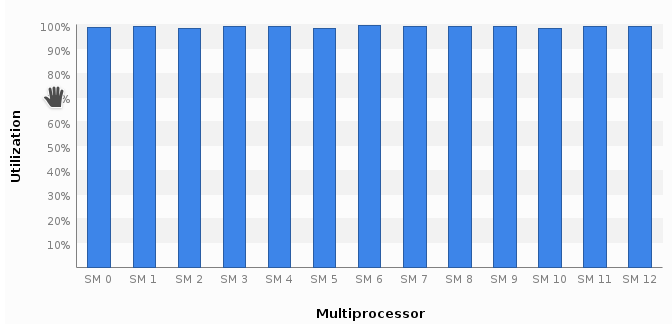
\includegraphics[width=0.8\textwidth,keepaspectratio]{%
    report/resources/mp_util.png}
  \end{center}
  \caption{Streaming Multiprocessor Auslastung}
  \label{fig:shm}
\end{figure}

Die Reparatur leerer Partitionen ist ebenfalls mittels Device-Code
implementiert, allerdings aufgrund der komplizierten Struktur der \texttt{sums}
und \texttt{counts} Arrays stark vereinfacht. Hier wird ein einzelner Thread
gestartet, der nacheinander in leere Partition die halbe akkumulierte Summe
einer anderen Partition überträgt. Dieser Prozess könnte auch auf dem Host
durchgeführt werden, wobei dann allerdings größerer Datenaustausch zwischen
Host und Device nötig wäre. Da dieser Abschnitt Performance-unkritisch ist, ist
die genaue Implementierung hier nicht entscheidend.

\subsection{Performance}

Der gewählte Ansatz liefert trotz suboptimaler Ausnutzung der Device-Hardware
gute Ergebnisse bezüglich der Ausführungszeit. Für eine kleine Pixel- Anzahl
überwiegt der durch das Starten von Kerneln und Kommunikation zwischen Host und
Device bedingte Overhead TODO. Aufgrund des deutlich größeren Anzahl paralleler
Prozessoren im Vergleich zur CPU lohnt sich dieser Overhead aber für das
getestete System bei zunehmender Problemgröße. Dies ist in
Abbildung~\ref{fig:all} gezeigt, die für eine Reihe von Problemgrößen den
Median der Ausführungszeit (je 100 Testläufe) für alle besprochenen
Implementierungen gegenüberstellt.

\begin{figure}[htbp]
  \centering
    \includesvg[width=\textwidth]{%
    report/resources/All_plot.png}
  \caption{Übersichts-Vergleich Ausführungszeiten (Median aus je 100 Testläufen)}
  \label{fig:all}
\end{figure}

\chapter{Nutzung des Repositorys}

Eine Anmerkung zu Beginn: Während der Entwicklung der
\texttt{CUDA}-Implementierung kam es zu mehreren Zeitpunkten zu
Programm-Fehlschlägen die durch Treiber-Probleme hervorgerufen wurden. Sollte
z.B. das \texttt{demo}-Programm mit einem durch \texttt{CUDA} hervorgerufenen
\texttt{unknown error} abstürzen hilft unter Umständen ein Neustart oder im
schlimmsten Fall eine Neuinstallation des \texttt{NVIDIA}-Treibers (mittels des
\texttt{CUDA-9.2}-Installers ab.

\section{Demo}

Wird aus dem Wurzelverzeichnis des Repositorys \texttt{make demo} ausgeführt,
werden die verschiedenen Implementierungen auf das Beispiel-Bild
\texttt{images/demo\_image.jpg} angewandt und die Ergebnisse dargestellt. Da
die initialen Partitions-Schwerpunkte zufällig gewählt werden kann es unter
Umständen vorkommen, dass die Ergebnisse leicht unterschiedlich ausfallen
(auch in Abhängigkeit der maximalen Anzahl von Iterationen).
Abbildung~\ref{img:demoresults} zeigt ein Beispiel

\begin{figure}[h]
\centering
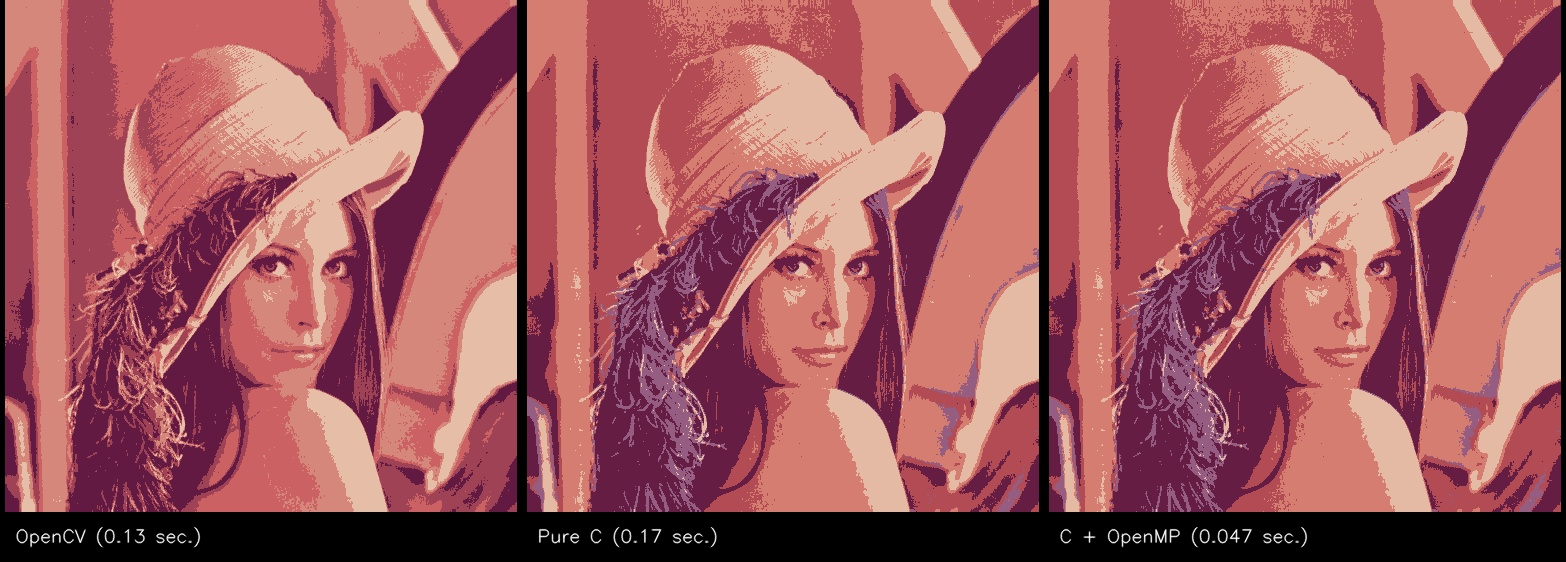
\includegraphics[width=\textwidth]{report/resources/demo_results.jpg}
\caption{Beispielhafte Demo Ergebnisse}
\label{img:demoresults}
\end{figure}

\section{Benchmark}

Bei Ausführung von \texttt{make benchmark} werden die Implementierungen
hingegen entsprechend der im \texttt{Makefile} gesetzten Parameter auf zufällig
generierte Bilder verschiedener Größen mit variierenden Partitions-Größen
angewandt und jeweils die Ausführungszeiten in \texttt{.csv} Datein im
\texttt{benchmarks} Verzeichnis protokolliert. Mit dem Python script
\texttt{tool/plot} können die Ergbenisse visualisiert werden, dazu muss
\texttt{./tool/plot benchmarks} ausgerufen werden (passiert bei Ausführung von
\texttt{make benchmark} automatisch). Die resultierenden Grafiken finden sich
unter \texttt{report/resources} und über diesen Bericht verteilt.

\chapter{Quellcode}

Alle genutzten Quellcode- und Build-Dateien:

\captionof{listing}{\texttt{kmeans.h}}
\inputminted{C}{c/include/kmeans.h}

\captionof{listing}{\texttt{kmeans\_config.h}}
\inputminted{C}{config/kmeans_config.h}

\captionof{listing}{\texttt{kmeans.c}}
\inputminted{C}{c/src/kmeans.c}

\captionof{listing}{\texttt{kmeans\_wrapper.h}}
\inputminted{C}{cpp/include/kmeans_wrapper.h}

\captionof{listing}{\texttt{kmeans\_wrapper.cc}}
\inputminted{C}{cpp/src/kmeans_wrapper.cc}

\captionof{listing}{\texttt{kmeans\_benchmark.cc}}
\inputminted{C}{cpp/src/kmeans_benchmark.cc}

\captionof{listing}{\texttt{kmeans\_demo.cc}}
\inputminted{C}{cpp/src/kmeans_demo.cc}

\captionof{listing}{\texttt{Makefile}}
\inputminted{make}{Makefile}

\begin{thebibliography}{1}
\bibitem[1]{bib:lloyd}
Lloyd., S. P. (1982). ``Least squares quantization in PCM''. IEEE Transactions
on Information Theory
\end{thebibliography}

\renewcommand\listoflistingscaption{Quellcodeverzeichnis}
\renewcommand{\listoflistings}{%
  \cleardoublepage
  \phantomsection
  \addcontentsline{toc}{chapter}{\listoflistingscaption}%
  \listof{listing}{\listoflistingscaption}%
}
\listoflistings

\end{document}
